\documentclass[titlepage]{article}
\usepackage{graphicx}

\begin{document}

\title{Experiment 0: Sensor Calibration and Linear Regression}
\author{Tian Ye \\ \\ UID: 704931660 \\ \\ TA: Wen Li Wen \\ \\ Lab Partner: Megan Wu \\ \\ Lab 8 Tuesday 6:00 PM}
\date{October 2nd, 2017}

\maketitle

\section*{Question 2}

Via Equation ii.23, we know that the definition of $\delta$\textit{a} follows the following ratio:

\[
\delta a = \sqrt{\bigg (\frac{\partial a}{\partial v}\delta v\bigg )^2 + \bigg (\frac{\partial a}{\partial t} \delta t\bigg )^2} \bigg |_{v\textsubscript{best}, t\textsubscript{best}}
\]

Therefore we find that $\frac{\partial a}{\partial v} = \frac{1}{t}$ and that  $\frac{\partial a}{\partial t} = \frac{-v}{t^2}$. Substituting these values back into the equation given above yields the following:

\[
\delta a = \sqrt{\bigg (\frac{1}{t}\delta v\bigg )^2 + \bigg (-\frac{v}{t^2}\delta t\bigg )^2} \bigg |_{v\textsubscript{best}, t\textsubscript{best}}
\]

\section*{Question 3}

Capstone will display up to 16 digits total; 15 after the decimal point. If the sensor precision is 4 digits, the actual measurement precision is 4 digits and digits 5 through 10 will fluctuate randomly, therefore having no meaning. However, turning down the sensor precision far enough so that there is no fluctuation at the same time also eliminates uncertainty, so some digits should be left so that uncertainty can be accounted for.

\section*{Question 4}

\begin{table}[!htbp]
\renewcommand{\arraystretch}{1.3}
\centering
\begin{tabular}{c|c|c}
    \hline
    \hline
    Mass of Weight  &  Force of Weight  &  Measured Voltage of Force Sensor\\
    \hline
    \hline

    50 grams   &   0.49 N  &  -0.08 volts\\
    \hline

    100 grams    &   0.98 N  &  -0.16 volts\\
    \hline

    200 grams  &  1.96 N  &  -0.31 volts\\
    \hline

    250 grams  &  2.45 N  &  -0.39 volts\\
    \hline

    300 grams  &  2.94 N  &  -0.46 volts\\
    \hline
\end{tabular}
\end{table}

\begin{figure}[ht]
    \centering
    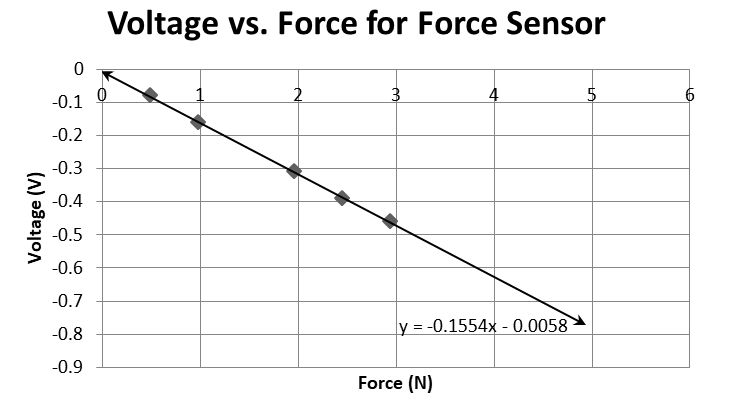
\includegraphics[width=6.0in]{LinReg.png}
    \caption{Voltage (V) displayed on Force Sensor plotted against Force (N) with linear fit line, as generated by Microsoft Excel. The sensor was zeroed after every test; the 250 gram and 300 gram masses were obtained by combining the 200 gram mass with a 50 gram and 100 gram mass, respectively. Force was obtained via multiplying the mass of each weight by the gravitational constant 9.8 m/{s}$^2$.}
    \label{fig:2}
\end{figure}

\clearpage

\section*{Question 5}

The result of the calibration creates a linear line with a negative slope that nearly passes through the origin. The voltage of the force sensor decreases as the mass, and consequently the force, increases. However, the fact that there is a nonzero y-intercept indicates that the taring procedure was not perfect, as otherwise the line would pass through the origin. The fact that it doesn't would imply that for a mass of 0, there is a force on the sensor. The values for the two variables \textit{a} and \textit{b} in the equation of \textit{V} = \textit{aF} + \textit{b} are:

\begin{center}
\textit{a} = (-0.155 $\pm$ 0.001) V/N
\end{center}

\begin{center}
\textit{b} = (-0.006 $\pm$ 0.003) V
\end{center}

\section*{Question 6}

The rewritten form of Voltage to Force following some algebraic manipulation is $F = cV + d$ where $c = \frac{1}{a}$ and $d = \frac{-b}{a}$. The uncertainty can then be found using the same Equation that was used in Question 2, in this case being

\[
\delta c = c\textsubscript{best}\bigg (\frac{\delta a}{a\textsubscript{best}}\bigg ) 
\]

\[
\delta d = d\textsubscript{best} \sqrt{\bigg (\frac{\delta b}{b\textsubscript{best}}\bigg )^2  + \bigg (\frac{\delta a}{a\textsubscript{best}}\bigg )^2}
\]

\begin{center}
Therefore the final values for $c$ and $d$ are
\end{center}

\begin{center}
$c = -6.45 \pm 0.04$ N/V
\end{center}

\begin{center}
$d = -0.04 \pm 0.02$ N
\end{center}

\section*{Question 7}

The discrepency in score is possible as the final grade in Physics 4AL is dependant on your score in relation to that of the rest of the class. In this case, the TA for Frankie Fivefingers most likely graded harder than that of Avril Armstrong. Consequently, while both students scored the same, Frankie scored comparatively better in relation to her peers in her class than did Avril in his. Thus, it can be concluded that the mean numerical score in Frankie Fivefingers's 4AL class was lower than that of Avril Armstrong's.

\end{document}
T